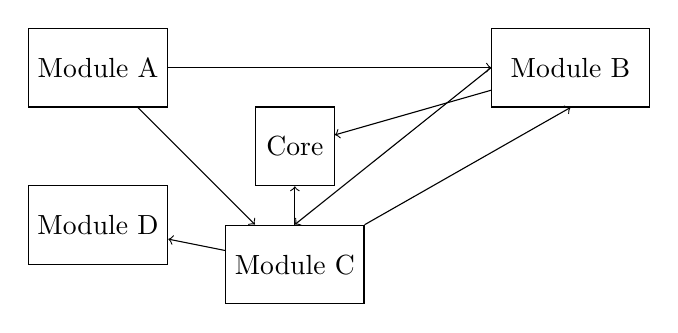
\begin{tikzpicture}
    \node (tabs) [rectangle, draw, minimum height=1cm, minimum width=1cm] at (0, 1) {Module A};
    \node (editor) [rectangle, draw, minimum height=1cm, minimum width=2cm] at (6, 1) {Module B};
    \node (fsa) [rectangle, draw, minimum height=1cm, minimum width=1cm] at (2.5, -1.5) {Module C};
    \node (cache) [rectangle, draw, minimum height=1cm, minimum width=1cm] at (0, -1) {Module D};
    \node (core) [rectangle, draw, minimum height=1cm, minimum width=1cm] at (2.5, 0) {Core};

    \draw[->] (tabs) to node[midway, above] {} (editor);
    \draw[->] (tabs) to node[midway, above] {} (fsa);
    \draw[->] (editor.west) to node[midway, above] {} (fsa.north);
    \draw[->] (editor) to node[midway, above] {} (core);
    \draw[->] (fsa) to node[midway, below] {} (editor.south);
    \draw[->] (fsa) to node[midway, above] {} (cache);
    \draw[->] (fsa) to node[midway, above] {} (core);
\end{tikzpicture}